\documentclass{proc}

\usepackage[margin=1in]{geometry}
\usepackage{graphicx}

\title{Including Graphics}
\author{Anuj Nair}
\date{}

\begin{document}
\maketitle

\section{Introduction}

Picture books are just \emph{better}

\subsection{Introduction Graphics}

  This is a banana in JPG.
  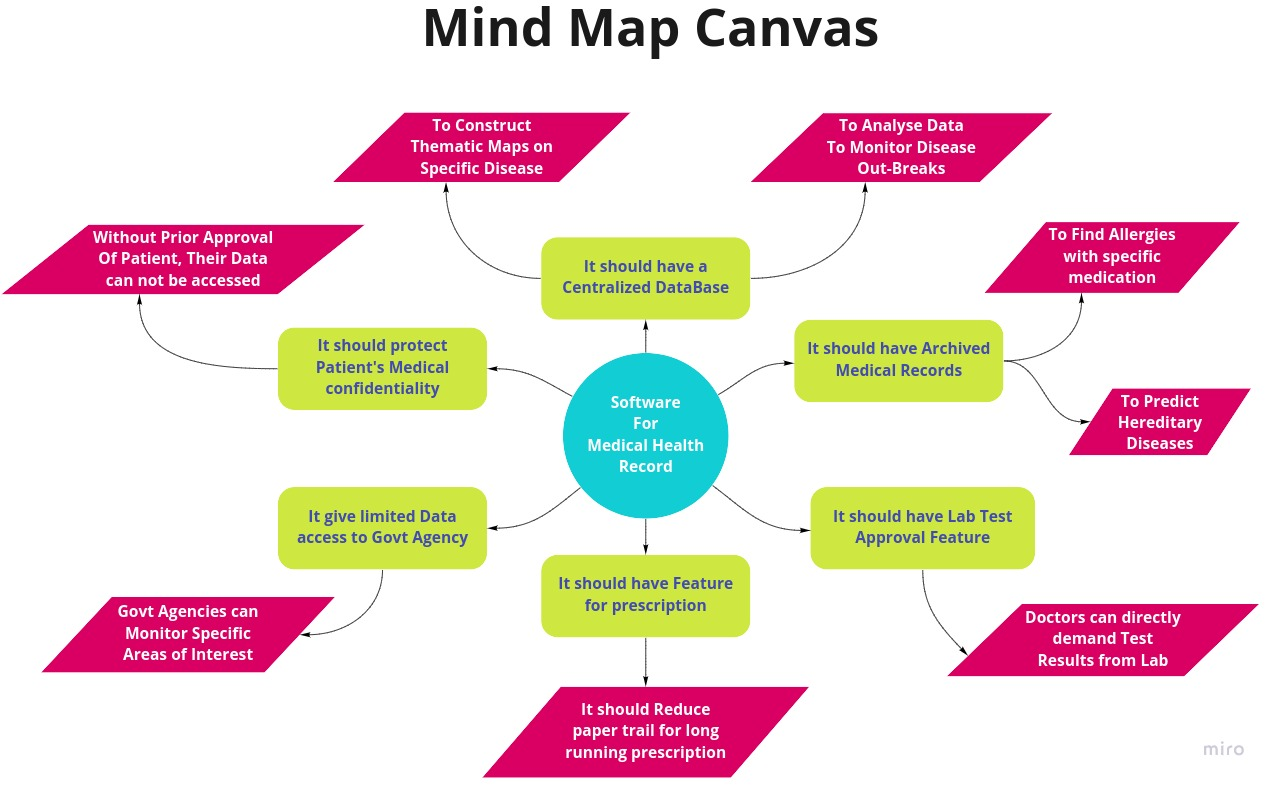
\includegraphics[width=2in]{me.jpg}

  This is a fish, in a chart, in PNG.
				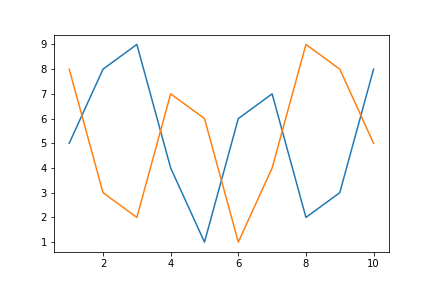
\includegraphics[width=2in]{graph.png}


   

\subsection{Float: Figure Environment}

  In my article, I want to include a JPG image of a banana. You can see this image in the Figure~\ref{fig:banana} .
  \begin{figure}[htbp]
    \begin{center}
				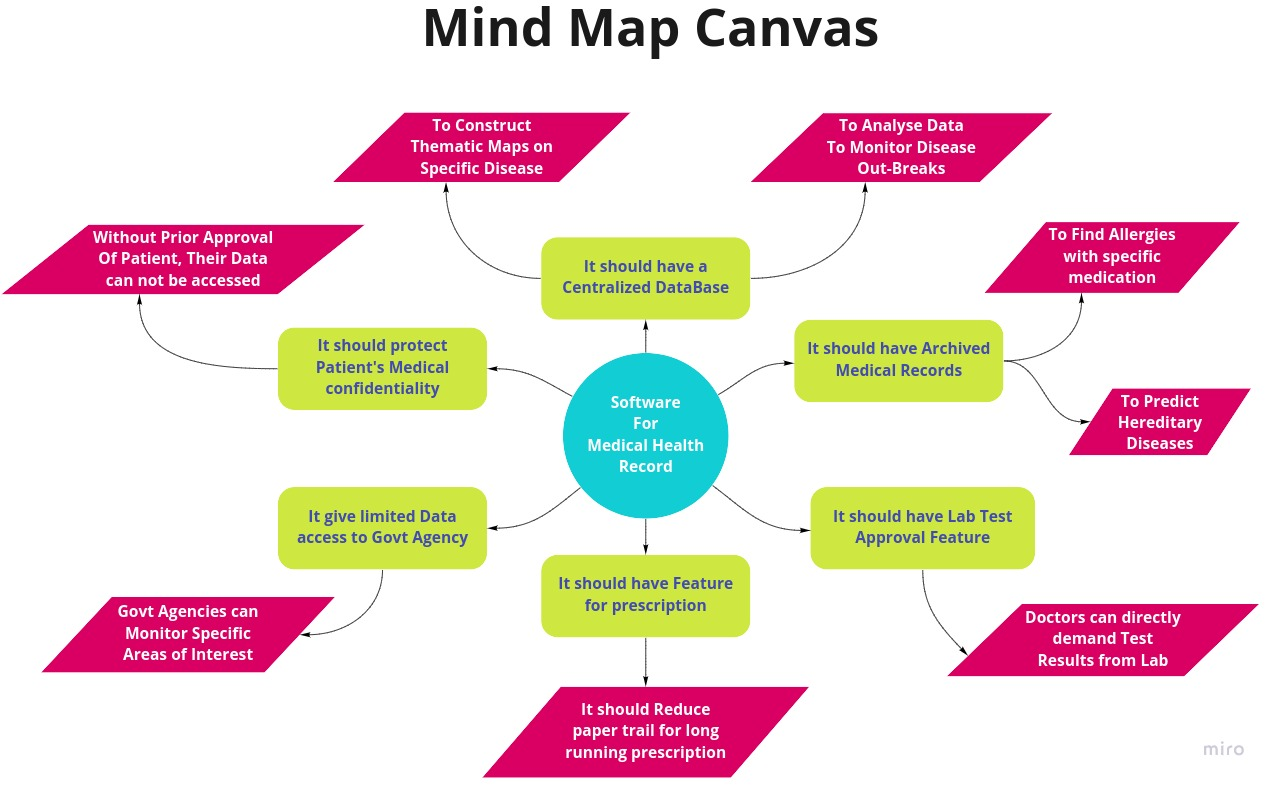
\includegraphics[width=2in]{me.jpg}
        \caption{This is a banana.}
        \label{fig:banana}
    \end{center}
  \end{figure}
  
  In my article, I want to include a PNG image of a chart that looks like a fish. You can see this image in the Figure~\ref{fig:fish} .
  \begin{figure}[htbp]
    \begin{center}
				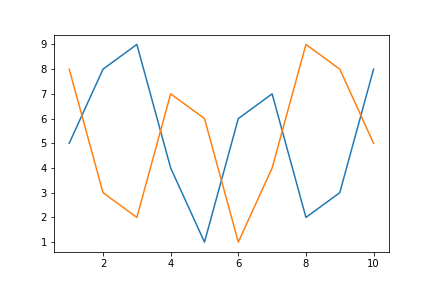
\includegraphics[width=2in]{graph.png}
        \caption{This is a chart that looks like a fish.}
        \label{fig:fish}
    \end{center}
  \end{figure}

     

\section{Conclusion}
  

\end{document}
